\chapter{基于时序建模的入侵检测}
本章节主要介绍如何对网络流量进行时序建模以实现入侵检测。网络流量是一种时序数据,网络入侵往往包含一系列的步骤,其进行顺序存在先后关系。入侵检测是基于异常进行检测,入侵行为往往会导致网络流量特征突然发生改变,通过进行时序分析可识别这些非正常的流量模式,实现对网络入侵的高效检测。

本章将会在前一章节已提取单个网络流量特征的前提下,进一步使用时序模型进行建模。

\section{基于RNN的时序建模}
RNN是进行时序建模的经典模型,过去大部分对网络入侵进行时序建模,都使用该模型及其对应的改进形式。该模型最大特点是内部维持隐状态,而输入序列会依次输入其中,隐状态会随输入而不断变化从而保留之前输入中的有效信息。
\subsection{标准RNN介绍}
\begin{figure}[htbp]
    \centering
    \includesvg[width=.67\textwidth,keepaspectratio]{img/sequence/rnn.svg}
    \caption{RNN的神经网络结构\cite{zhang2023dive}}
    \label{fig:rnn_struct}
\end{figure}
如图\ref{fig:rnn_struct}示,最基础的循环神经网络在t时刻只有一个隐藏状态$\mathbf{H}_{t}$,该隐藏状态由上一时刻的隐藏状态$\mathbf{H}_{t-1}$与当前时刻的输入$\mathbf{X}_{t}$决定,现在每一时刻的输出只与当前时刻的隐藏态有关,具体计算过程如下:
\begin{equation}
\begin{aligned}
\mathbf{H}_{t} &= \sigma(\mathbf{W}_{\mathrm{h}} \cdot [\mathbf{H}_{t-1}, \mathbf{X}_t] + \mathbf{b}_{\mathrm{h}})\\
\mathbf{O}_{t} &= \sigma(\mathbf{W}_{\mathrm{o}}\mathbf{H}_{t} + \mathbf{b}_{\mathrm{o}})\\
\end{aligned}
\end{equation}
其中$\mathbf{W}_{hh}$ 是前一时刻隐藏状态对当前时刻隐藏状态的权重矩阵,$\mathbf{W}_{xh}$ 是当前时刻输入到当前时刻隐藏状态之间的权重矩阵,$\mathbf{b}_{h}$ 是隐藏层的偏置向量,$\sigma$ 是激活函数,循环神经网络最常用的激活函数是tanh,其特点是输出范围在-1到1,均值为0。输出范围中心化有利于下一层的输入的分布保持均衡,从而提高模型稳定性。

当神经元计算得到当前时刻隐藏状态时就可计算当前时刻的输出,因为输出只与隐藏状态有关,其中$\mathbf{W}_{ho}$ 是当前时刻隐藏状态到当前时刻输出之间的权重矩阵,$\mathbf{b}_{o}$ 是输出层的偏置向量。

在标准RNN中,信息从前一时刻传至当前时刻,需要经过矩阵变换以及激活函数激活,多次传递会造成梯度消失或梯度爆炸,因此网络难以学习长距离时序依赖关系。

\subsection{长短期记忆网络}

\begin{figure}[hbtp]
    \centering
    \includesvg[width=.67\textwidth,keepaspectratio]{img/sequence/lstm.svg}
    \caption{LSTM的神经网络结构\cite{zhang2023dive}}
    \label{fig:lstm_struct}
\end{figure}

如图\ref{fig:lstm_struct}示,LSTM针对标准RNN存在的问题,使用三个门控机制(遗忘门$\mathbf{F}_t$、输入门$\mathbf{F}_t$、输出门$\mathbf{O}_t$)控制信息流动,同时引入了长期记忆单元$\mathbf{C}$,这些门控机制决定LSTM需要记忆,需要忘记以及需要输出的信息,从而解决梯度爆炸或消失的问题,其具体计算过程如下:

\begin{enumerate}
    \item 遗忘门$\mathbf{F}_t$决定需要记忆与忘记的信息。
    \item 输入门$\mathbf{I}_t$决定当前时刻输入$X_t$中需要保留到记忆单元$\mathbf{C}$中的信息。
    \item 输出门$\mathbf{O}_t$决定当前时刻输出值。
    \item 候选记忆 $\mathbf{C}'_t$  是从短期记忆中需要被转移至长期记忆的信息。 
    \item 记忆单元$\mathbf{C}_t$由候选记忆以及上一时刻的记忆单元信息更新
    \item 隐状态$\mathbf{H}_t$,由输出门和记忆单元决定
\end{enumerate}

\begin{equation}
\begin{aligned} 
\mathbf{F}_t &= \sigma(\mathbf{W}_{\mathrm{f}} \cdot [\mathbf{H}_{t-1}, X_t] + \mathbf{b}_{\mathrm{f}})\\ 
\mathbf{I}_t &= \sigma(\mathbf{W}_{\mathrm{i}} \cdot [\mathbf{H}_{t-1}, X_t] + \mathbf{b}_{\mathrm{i}})\\ 
\mathbf{O}_t &= \sigma(\mathbf{W}_{\mathrm{o}} \cdot [\mathbf{H}_{t-1}, X_t] + \mathbf{b}_{\mathrm{o}})\\ 
\mathbf{C}'_t &= \tanh(\mathbf{W}_C \cdot [\mathbf{H}_{t-1}, X_t] + \mathbf{b}_C)\\ 
\mathbf{C}_t &= \mathbf{F}_t \ast \mathbf{C}_{t-1} + \mathbf{I}_t \ast \mathbf{C}'_t\\ 
\mathbf{H}_t &= \mathbf{O}_t \ast \tanh(\mathbf{C}_t)\\ 
\end{aligned}
\end{equation}

其中,$\sigma$为sigmoid函数,将门控的输出值的大小控制在0和1之间,$\ast$表示Hadamard积,即元素对元素的乘积;$W$和$b$分别代表映射矩阵和对应的偏置向量,下标$f$、$i$、$C$和$o$分别表示遗忘门、输入门、候选长期记忆和输出门。

LSTM通过门控机制一定程度上解决了长序列中的梯度爆炸与消失问题,但其结构过于复杂,每个神经元内的计算步骤多,消耗计算资源大。

\subsection{基于门控神经元的循环神经网络}
\begin{figure}[htbp]
    \centering
    \includesvg[width=.67\textwidth,keepaspectratio]{img/sequence/gru.svg}
    \caption{GRU的神经网络结构\cite{zhang2023dive}}
    \label{fig:gru_struct}
\end{figure}

如图\ref{fig:gru_struct}示,GRU对LSTM进行一定程度的简化,在避免梯度异常的同时降低了模型的计算量。其使用两个门控机制(重置门$\mathbf{R}_t$、更新门$\mathbf{Z}_t$)进行信息选择,主要更新过程如下:
\begin{enumerate}
    \item 更新门$\mathbf{Z}_t$控制状态更新时前一时刻隐状态$\mathbf{H}_{t-1}$中信息的保留。
    \item 重置门$\mathbf{R}_t$决定计算候选隐藏状态$\tilde{\mathbf{H}}_t$ 时对前一时刻隐藏状态$\mathbf{H}_{t-1}$的参考程度。
    \item 候选隐藏状态$\tilde{\mathbf{H}}_t$ 由前一时刻隐藏状态$\mathbf{H}_{t-1}$和当前时刻输入$\mathbf{X}_t$决定。
    \item 最终隐藏状态$\mathbf{H}_t$由前一时刻隐藏状态$\mathbf{H}_{t-1}$以及当前时刻候选隐藏状态$\tilde{\mathbf{H}}_t$ 决定。
\end{enumerate}

\begin{equation}
    \begin{aligned}
        \mathbf{Z}_t &= \sigma(\mathbf{W}_{\mathrm{z}} \cdot [\mathbf{H}_{t-1}, \mathbf{X}_t] + \mathbf{b}_{\mathrm{z}})\\
        \mathbf{R}_t &= \sigma(\mathbf{W}_r \cdot [\mathbf{H}_{t-1}, \mathbf{X}_t] + \mathbf{b}_{\mathrm{r}})\\
        \tilde{\mathbf{H}}_t &= \tanh(\mathbf{W}_{\mathrm{h}} \cdot [\mathbf{R}_t \ast \mathbf{H}_{t-1}, \mathbf{X}_t] + \mathbf{b}_{\mathrm{h}})\\
        \mathbf{H}_t &= \mathbf{Z}_t \ast \mathbf{H}_{t-1} + (1 - \mathbf{Z}_t) \ast \tilde{\mathbf{H}}_t
    \end{aligned}   
\end{equation}

其中,$\sigma$与LSTM中的门控机制激活函数相同为sigmoid;$W$和$b$分别表示投影矩阵和对应的偏置向量,下标$z$、$r$和$h$分别代表更新门、重置门和候选隐藏状态。

GRU简化了LSTM的门控机制,减少了模型的参数量与计算量,虽然其长序列建模能力弱于LSTM,但在计算资源有限的情况下可作为其近似替代。

\section{基于Transformer的时序建模}
Transformer架构已在上一章节进行详细介绍。该架构有很多特点,上一章节主要利用其可伸缩性以及灵活性实现多模态建模,且多模态模型在获得数据各属性文本描述的情况下,可兼容任何格式数据集。

本章将继续利用该架构进行时序建模。相比上一节介绍的基于RNN及改进形式的时序建模,基于Transformer的时序建模在网络入侵领域检测领域更合适,特别是针对一些时间跨度较大的网络攻击方式。在KDDCUP-99数据集中的Slowloris就是一种经典的低速攻击,通过缓慢发送HTTP请求,实现占有服务器资源的目的。较新的勒索软件攻击,也是一种需要进行长距离建模的网络入侵,它包含多个步骤,从开始渗透到最终完成对文件的加密并发送密钥,会间隔较长时间。

\section{基于时序建模的入侵检测模型}
在上一章提出了一种基于文本辅助的分类模型,模型包括编码与分类两部分,文章将会继续使用其中编码部分$F_{encoder}$,编码器将任意格式的网络流量特征映射为128维的向量。另一方面为方便模型分析与对比,本章将会使用线性编码器,该编码器实际为投影矩阵$Porj_{encoder}$,可将流量特征线性映射至128维。

在处理网络数据包时需考虑每个数据包本身的上下文无关特征,以及其在时间序列中的上下文信息,本节采用两阶段的处理流程。第一步,通过一定的特征提取方法(非线性编码或线性编码)获得每个数据包的上下文无关特征$\mathbf{z}_{\mathrm{cls}}$,该特征为一定长向量。第二步,为了捕捉时间序列中的上下文关联性,分别使用基于RNN或使用Transformer的时序的模型进行上下文建模。

基于Transformer的时序建模过程如算法\ref{alg:transformer_serial}示。

\begin{algorithm}[htb]
\caption{四层Transformer时序建模算法}
\begin{algorithmic}
\REQUIRE 定长序列 $S$,其中 $S$ 是一个 $N \times 128$ 的矩阵,$N$ 表示序列长度
\ENSURE 等长序列 $S'$,输出序列也是一个 $N \times 128$ 的矩阵

\STATE 分割 $S$ 为若干个长度为 $L$ 的序列片段 $\{S_1, S_2, \ldots, S_k\}$
\STATE 对每个序列片段 $S_i$,引入可学习的令牌 $\mathbf{T} = \{\mathbf{t}_1, \mathbf{t}_2, \ldots, \mathbf{t}_m\}$
\STATE 初始化四层Transformer模型 $Trans_1, Trans_2, Trans_3, Trans_4$
\FOR{$i = 1$ 到 $4$}
    \IF{$i == 1$}
        \STATE $input \gets [\mathbf{T}; S_i]$  \COMMENT{第一层的输入包括令牌和序列片段}
    \ELSE
        \STATE $input \gets output$  \COMMENT{后续层的输入为前一层的输出}
    \ENDIF
    \STATE $output \gets Trans_i(input)$ \COMMENT{使用Transformer层处理输入}
    \IF{$i == 4$}
        \STATE 移除输入中的可学习令牌 $\mathbf{T}$,保留序列信息得到 $S'$
    \ENDIF
\ENDFOR
\RETURN $S'$
\end{algorithmic}
\label{alg:transformer_serial}
\end{algorithm}

本章同样使用四层Transformer对数据流量进行时序建模。与RNN不同Transformer的注意力机制中计算复杂度与序列的长度呈平方关系而不是线性关系,因此在算法的第1步会将网络流量切为长度相同的短片段,若数据预处理中已对数据进行分割,则此步不必进行。对于分割后的子序列,算法会在序列头部加入特殊向量,该向量用于表示整个序列的上下文信息。

在算法的执行过程中,Transformer的每一层输入都会作为下一层的输出,以此实现模型对流量特征的提取。在最后一层算法会移除之前加入的头部特殊向量,得到与源序列等长部分并输出。



\begin{enumerate}
\item 时间序列分段
   
   对于一个时间序列数据,例如由网络数据包组成的序列,首先将其划分为长度相同的子序列,这些子序列不应该有重叠。设定一个序列片段的长度为 $L$(也就是窗口大小),则原时间序列可以被分为若干个长度为 $L$ 的序列片段:

   \begin{equation}
          \mathbf{S}_i = \{\mathbf{z}_{\mathrm{cls}}^{(i*L)}, \mathbf{z}_{\mathrm{cls}}^{(i*L+1)}, \ldots, \mathbf{z}_{\mathrm{cls}}^{(i*L+L-1)}\}
   \end{equation}

   其中,$\mathbf{S}_i$ 表示第 $i$ 个序列片段,$\mathbf{z}_{\mathrm{cls}}^{(j)}$ 表示第 $j$ 个数据包的上下文无关特征。

\item 引入可学习的令牌

   在输入Transformer模型之前,引入一系列可学习的令牌,可以捕获和存储全局信息。设定这些可学习的令牌集合为 $\mathbf{T} = \{\mathbf{t}_1, \mathbf{t}_2, \ldots, \mathbf{t}_m\}$,其中 $m$ 是可学习令牌的数量。这些令牌被初始化,并在训练过程中与其他参数一起更新。

\item Transformer模型

   使用一个4层的Transformer结构来处理上述拼接后的序列数据。Transformer的输入是编码器头生成的特征向量序列加上可学习的令牌。设Transformer的输出为 $\mathbf{O}$:

   \begin{equation}
   \mathbf{O} = {\mathrm{Transformer}}([\mathbf{T}; \mathbf{S}_i])
   \end{equation}

   其中,$[\mathbf{T}; \mathbf{S}_i]$ 表示令牌和序列片段的拼接。

\item 移除令牌

   在Transformer模型处理完毕后,移除步骤2中添加的可学习令牌,只保留与原始数据包对应的输出部分。这样得到的输出序列 $\mathbf{O'}$ 只包含了来自原始序列片段的信息:

   \begin{equation}
   \mathbf{O'} = \mathbf{O} \setminus \mathbf{T}
   \end{equation}
\end{enumerate}

通过以上两种时序模型可在保留数据包的独立特征的同时,学习到序列中的上下文关联。因而模型在对数据包进行分析时可通过上下文信息进行更准确的判断。

\section{实验结果}
本章是在上一章的基础上进行时序建模探索,前一章节的预实验已证明使用时序模型可提高模型的拟合能力。本小节将会对基于时序建模的模型性能进行进一步实验分析。第一步对最简单的时序模型即使用线性编码器的不同时序模型进行研究,实验平台和实验参数与上一章保持一致,只有模型不同。本小节所用线性编码器即为投影矩阵。实验结果如表\ref{tab:none-seq}示。
\begin{table}[!ht]
    \centering
    \caption{基于线性编码器的时序模型CIC-IDS2017数据集上的表现}
    \begin{adjustbox}{max width=.75\textwidth}
    \begin{tabular}{llllll}
    \toprule
        衡量指标 & 实验编号 & exp1(a) & exp2(b)  & exp3(c) & exp4(d)\\ \midrule
        时序建模方式 & ~ & RNN & LSTM & GRU  & Transformer  \\ 
        recall & BENIGN & \textbf{1} & \textbf{1} & \textbf{1} & 0.9907 \\
        recall & Web-Attacks & 0 & 0 & 0 & \textbf{0.9345} \\
        recall & Botnet & 0 & 0 & 0 & \textbf{0.8388} \\
        recall & PortScan & 0 & 0 & 0 & \textbf{0.9971} \\
        recall & Unknown & 0 & 0 & 0 & \textbf{0.8571} \\
        recall & Denial-of-Service & 0 & 0 & 0 & \textbf{0.9949} \\
        recall & Brute-force-attack & 0 & 0 & 0 & \textbf{0.9537} \\
        acc & all & 0.8037 & 0.8037 & 0.8038 & \textbf{0.9913} \\

    \bottomrule
    \end{tabular}
    \end{adjustbox}
    \label{tab:none-seq}
\end{table}

分析可得,基于RNN的时序模型均发生过拟合,除正常类别外所有其他类别召回率均为0,仅输出样本个数最多的类别即正常类别。基于Transformer架构的时序模型则正常输出,对正常样本的识别能力弱于对拒绝服务、端口扫描等样本数较多的恶意类别。

以上的实验结果说明,仅使用时序模型进行建模,并不能充分提取网络特征,因此需要将时序模型与上一章提出的通用编码器相结合,组合后的实验结果如表\ref{tab:tr-seq}示。

\begin{table}[!ht]
    \centering
    \caption{基于通用编码器的时序模型在CIC-IDS2017数据集上的表现}
    \begin{adjustbox}{max width=.75\textwidth}
    \begin{tabular}{llllll}
    \toprule
        衡量指标 & 实验编号 & exp1(a) & exp2(b)  & exp3(c) & exp4(d)\\ \midrule
        时序建模方式 & ~ & GRU & LSTM & RNN  & Transformer  \\ 
        precision & BENIGN & 0.9995  & 0.9992  & 0.9993  & \textbf{0.9996} \\
        precision & Web-Attacks & 0.7417  & 0.5573  & 0.7006  & \textbf{0.9130} \\
        precision & Botnet & 0.4693  & 0.3876  & 0.2663  & \textbf{0.6538} \\
        precision & PortScan & \textbf{0.9942}  & 0.9895  & 0.9901  & 0.9924 \\
        precision & Unknown & 0.0284  & 0.0045  & 0.0211  & \textbf{0.3158} \\
        precision & Denial-of-Service & 0.9955  & 0.9887  & 0.9931  & \textbf{0.9985} \\
        precision & Brute-force-attack & 0.8825  & 0.7444  & 0.8167  & \textbf{0.9317} \\
        recall & BENIGN & 0.9967  & 0.9931  & 0.9939  & \textbf{0.9983} \\
        recall & Web-Attacks & 0.9680  & 0.9485  & 0.9582  & \textbf{0.9791} \\
        recall & Botnet & 0.9670  & 0.9414  & 0.9597  & \textbf{0.9890} \\
        recall & PortScan & \textbf{0.9987}  & 0.9978  & 0.9979  & 0.9984 \\
        recall & Unknown & 0.5714  & 0.1429  & \textbf{0.8571}  & \textbf{0.8571} \\
        recall & Denial-of-Service & 0.9976  & 0.9964  & 0.9969  & \textbf{0.9987} \\
        recall & Brute-force-attack & 0.9951  & 0.9944  & 0.9893  & \textbf{0.9966} \\
        f1 & BENIGN & 0.9981  & 0.9961  & 0.9966  & \textbf{0.9989} \\
        f1 & Web-Attacks & 0.8399  & 0.7021  & 0.8094  & \textbf{0.9449} \\
        f1 & Botnet & 0.6320  & 0.5491  & 0.4169  & \textbf{0.7872} \\
        f1 & PortScan & \textbf{0.9964}  & 0.9936  & 0.9940  & 0.9954 \\
        f1 & Unknown & 0.0541  & 0.0088  & 0.0412  & \textbf{0.4615} \\
        f1 & Denial-of-Service & 0.9965  & 0.9926  & 0.9950  & \textbf{0.9986} \\
        f1 & Brute-force-attack & 0.9354  & 0.8514  & 0.8948  & \textbf{0.9631} \\
        acc & all & 0.9969  & 0.9937  & 0.9945  & \textbf{0.9983} \\
    \bottomrule
    \end{tabular}
    \end{adjustbox}
    \label{tab:tr-seq}
\end{table}

将表\ref{tab:tr-seq}与表\ref{tab:none-seq}对比可知,引入通用编码器,避免了模型过拟合。其中三种基于RNN都是时序网络架构均能实现正常输出。其中基于Transformer架构的时序模型分类准确度最高为99.83\%,效果最差的是LSTM
,仅为99.37\%。基于Transformer架构的时序模型在几乎全部类别的分类结果上均优于其他模型,除了端口扫描。所有基于RNN的网络结构中,效果最好的是基于GRU的网络,在端口扫描上的三项指标均优于Transformer架构。

如图\ref{fig:tr-serial_confusion_matrix}示,基于Transformer的时序建模与基于RNN的时序建模在识别小样本类别上有比较高的准确率。基于LSTM的时序模型对小样本类别,识别能力最差,仅能识别约14\%的样本。

\begin{figure}[htbp] % 创建一个新的figure环境
\centering % 居中对齐所有的子图

\subfloat[基于RNN的时序模型]{ % 插入第二个子图及其标题
\begin{minipage}{0.435\linewidth}
\centering
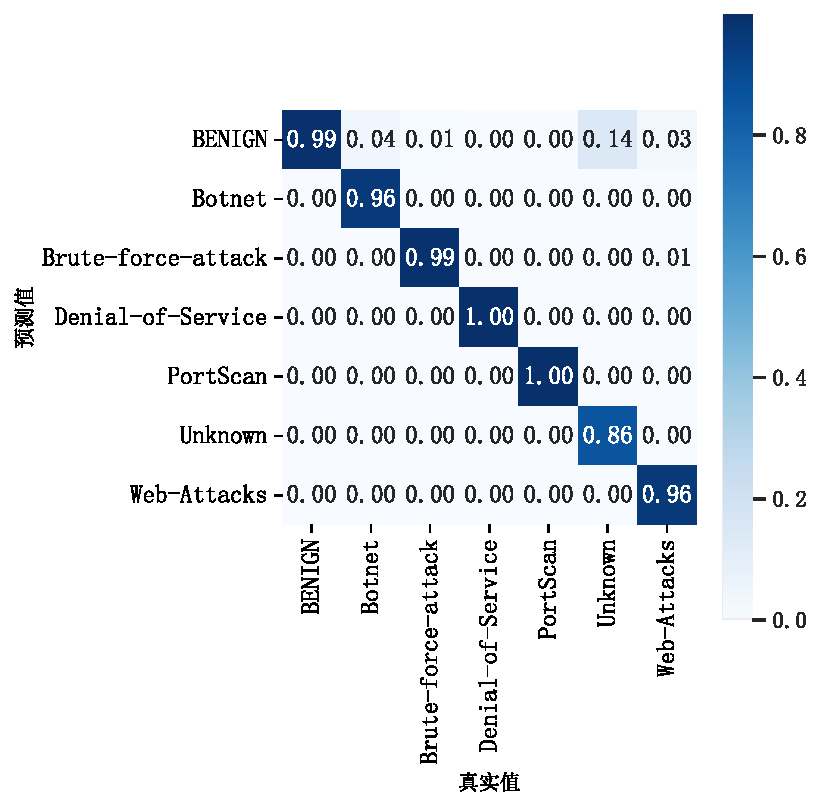
\includegraphics[width=1\linewidth]{img/exp2/3tr-rnn_confusion_matrix.pdf}
\label{fig:3tr-rnn_confusion_matrix}
\end{minipage}
}
\subfloat[基于LSTM的时序模型]{ % 插入第三个子图及其标题
\begin{minipage}{0.435\linewidth}
\centering
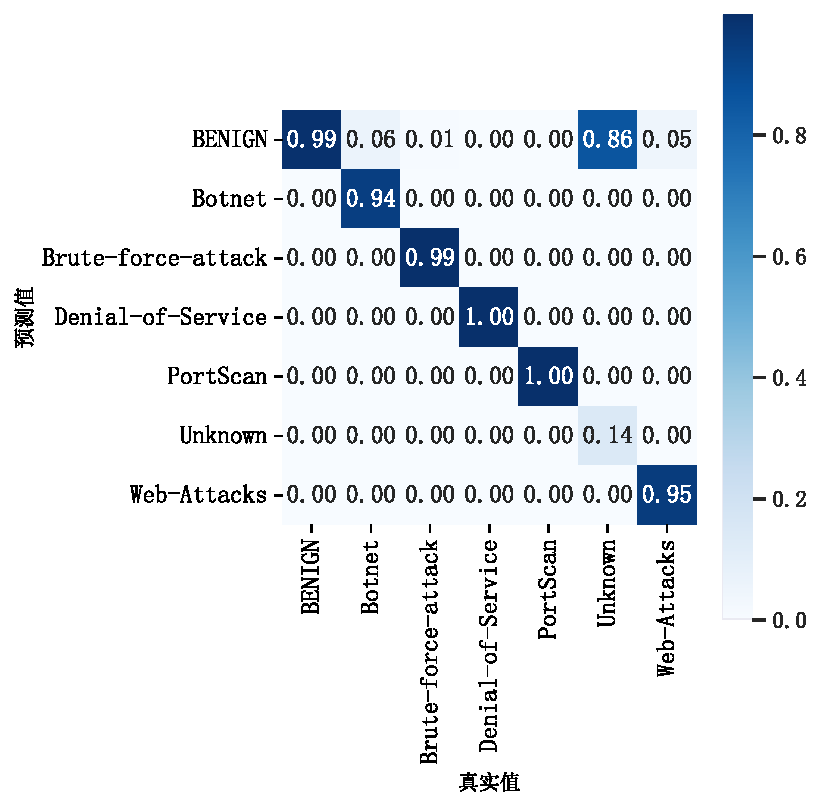
\includegraphics[width=1\linewidth]{img/exp2/5tr-lstm_confusion_matrix.pdf}
\label{fig:5tr-lstm_confusion_matrix}
\end{minipage}%
}

\subfloat[基于GRU的时序模型]{ % 插入第四个子图及其标题
\begin{minipage}{0.435\linewidth}
\centering
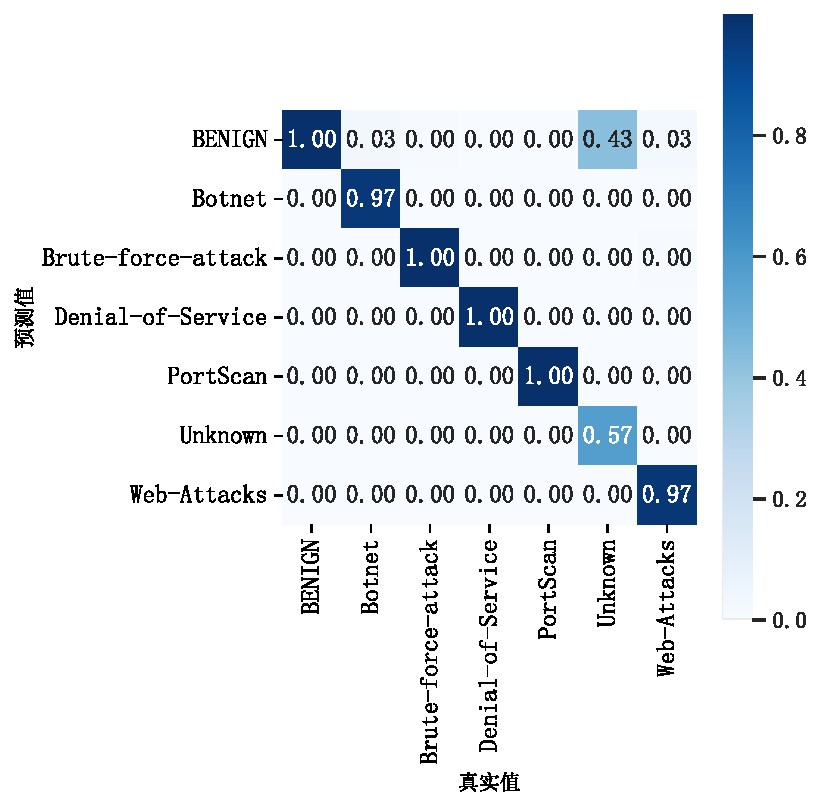
\includegraphics[width=1\linewidth]{img/exp2/7tr-gru_confusion_matrix.pdf}
\label{fig:7tr-gru_confusion_matrix}
\end{minipage}
}
\subfloat[基于Traansformer的时序模型]{ % 插入第四个子图及其标题
\begin{minipage}{0.435\linewidth}
\centering
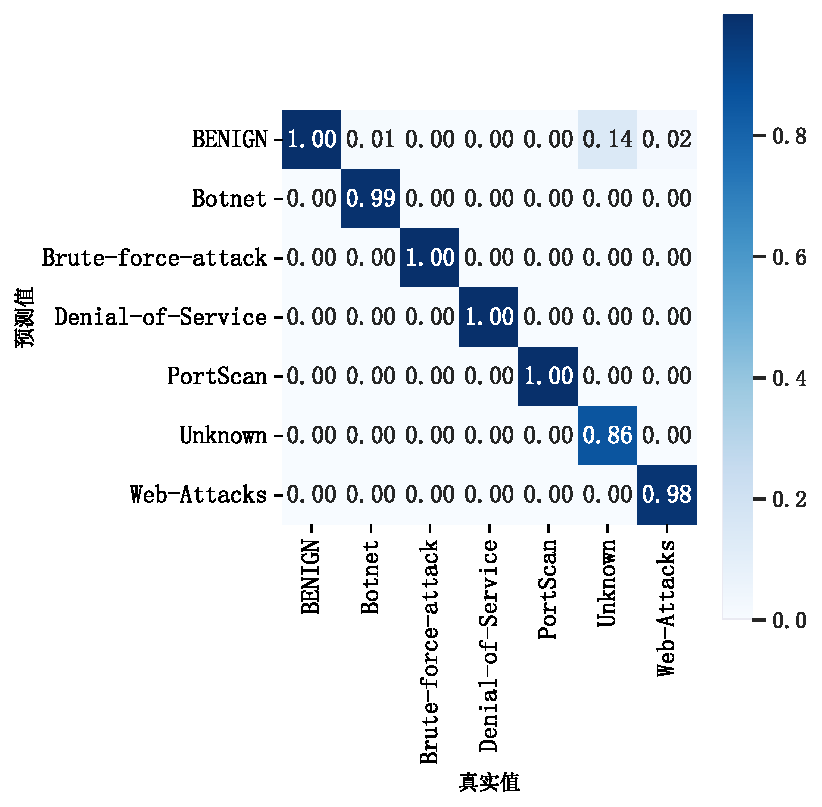
\includegraphics[width=1\linewidth]{img/exp2/1tr-tr_confusion_matrix.pdf}
\label{fig:1tr-tr_confusion_matrix}
\end{minipage}
}
\caption{使用通用编码器编码的不同时序模型混淆矩阵} % 整个figure的标题
\label{fig:tr-serial_confusion_matrix}
\end{figure}

LSTM有更复杂的门控结构,大部分任务上其性能要比GRU好。在网络入侵检测任务上性能差可能是在极度不均衡数据集上训练模型时,很难将LSTM调整到最适合的参数,而结构较为简单的GRU调节起来也较LSTM容易,可更快达到最优状态。标准RNN因其原本的特性难以对长序列建模而性能弱于GRU。

Transformer中的注意力机制在帮助模型实现长距建模的同时也提供了一种良好的可视化手段。在注意力机制中,每个头都有独立的注意力矩阵,为方便可视化,本小节仅取所有头的均值作为平均注意力值,该值反映了同一序列中两个位置的相关程度。如图\ref{fig:serial_att}示较浅层的注意力分数往往表现为平均,而最后一层的注意力分数最亮与最暗的值较多。这说明通过注意力机制模型,原有的预测被不断纠正,并最终接近实际标签。

\begin{figure}[htbp] % 创建一个新的figure环境
\centering % 居中对齐所有的子图

\subfloat[第1层注意力矩阵]{ % 插入第二个子图及其标题
\begin{minipage}{0.5\linewidth}
\centering
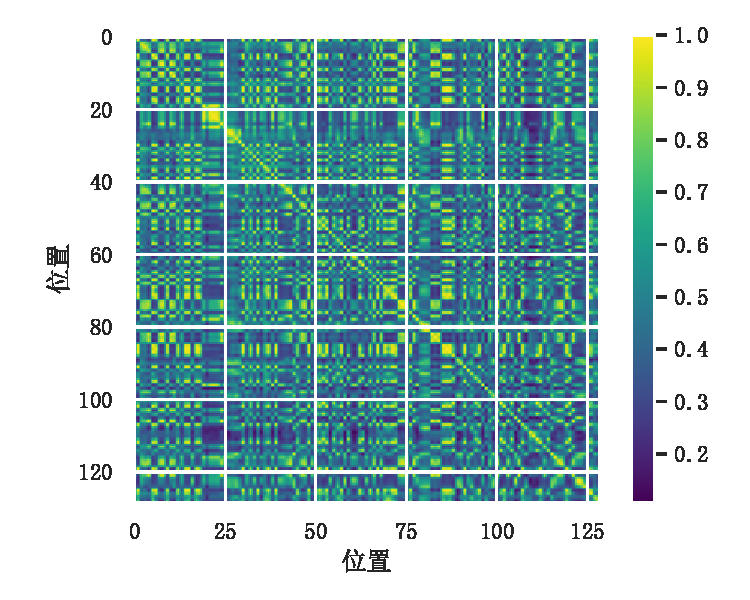
\includegraphics[width=1\linewidth]{img/sequence/att0.pdf}
\label{fig:serial_att_1}
\end{minipage}
}
\subfloat[第4层注意力矩阵]{ % 插入第三个子图及其标题
\begin{minipage}{0.5\linewidth}
\centering
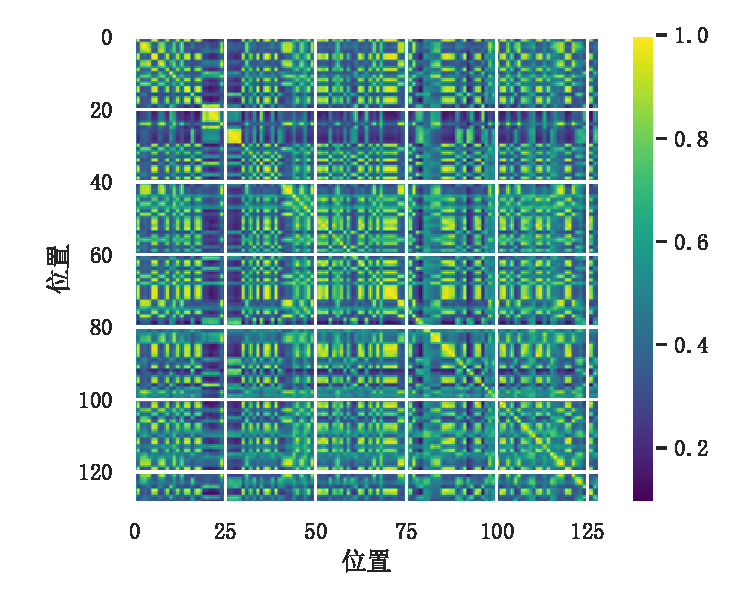
\includegraphics[width=1\linewidth]{img/sequence/att3.pdf}
\label{fig:serial_att_4}
\end{minipage}%
}

\caption{基于Transformer的时序模型注意力可视化} % 整个figure的标题
\label{fig:serial_att}
\end{figure}

实验证明对网络流量使用上一章提出的语言辅助编码器进行统一编码后,再使用时序模型进行时序建模,可得到更高的准确率。具体建模过程如图\ref{fig:overview}示。
\begin{figure}[htb]
    \centering
    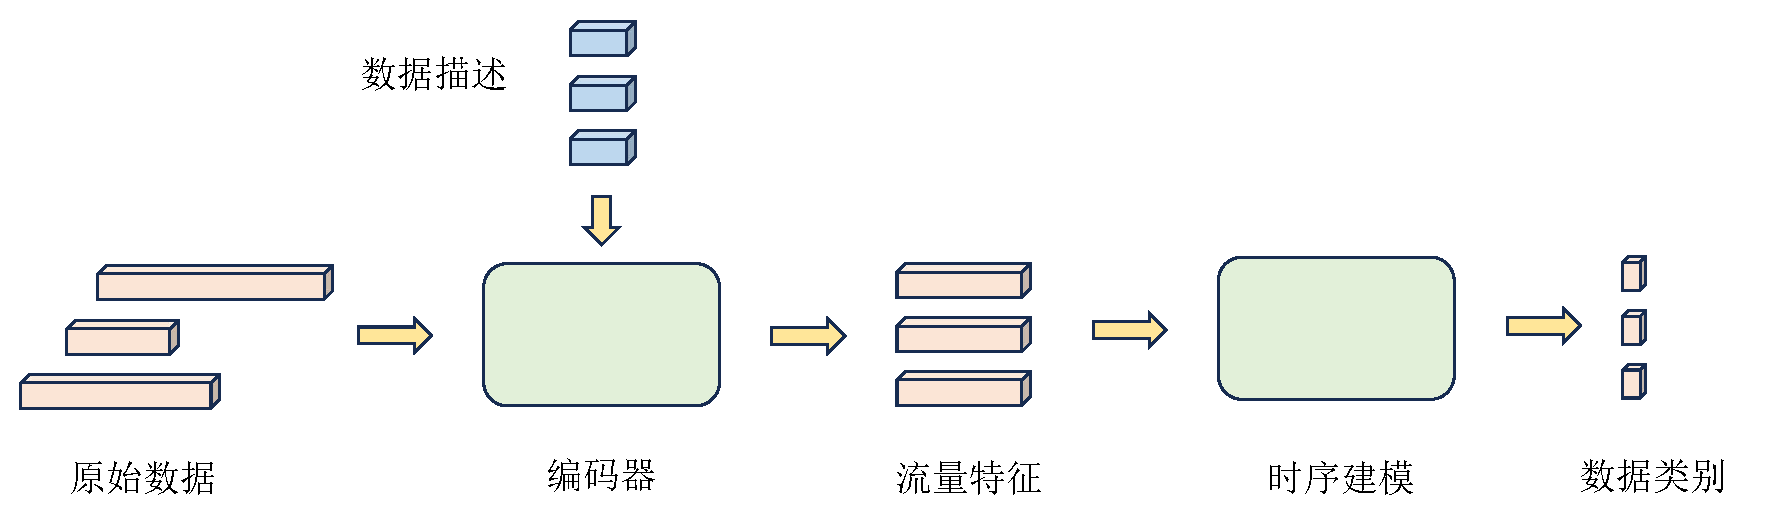
\includegraphics[width=\textwidth,height=\textheight,keepaspectratio]{img/overview.pdf}
    \caption{基于语言辅助编码器的时序模型}
    \label{fig:overview}
\end{figure}
网络由两部分组成,在第1步对不同类型的数据,结合数据本身的特征和对特征的文字描述,使用编码器形成对这些数据的编码即流量特征。第二步是结合数据的上下文特征进行时序建模,并根据建模结果得到这些数据对应的类别。

与近期方法比较如表\ref{tab:trm_cic2017_compare}示,本章提出的方法在CIC-IDS2017数据集上具有一定的先进性。

\begin{table}[htb]
    \centering
    \caption{CIC-IDS2017数据集上与其他方法对比}
    \begin{tabular}{lll}
    \toprule
        模型 & 分类数 & 准确率 \\ \midrule
        本章提出的方法 & 7 & 99.83\% \\ 
        LUCID\cite{10.1109/TNSM.2020.2971776}& 2 & 99.66\% \\ 
        CNN+LSTM\cite{10.1109/CCWC.2019.8666588}& 2 & 98.44\% \\
        MECNN\cite{10.1016/j.knosys.2022.108505}& 7& 99.73\%\\ 
        \bottomrule
    \end{tabular}
    \label{tab:trm_cic2017_compare}
\end{table}

\section{本章小结}
本章对基于时序建模的入侵检测模型进行研究,并对不同结构的时序模型进行实验,分析其在 CIC-IDS2017数据集上的性能与效果。

在本章节的开始对经典RNN及其改进形式进行了介绍,随后提出了基于Transformer的时序检测模型。通过三种RNN与Transformer进行对比发现,基于Transformer入侵检测模型在CIC-IDS2017这种数据分布极不均衡的数据集上具有较好的拟合能力。其他三种RNN出现了过拟合现象,对于全部样本仅输出数量最多的类别即正常类别,而基于Transformer性能表现弱于上一章节提出的针对单个流量的多模态入侵检测。

以上4种模型加入前一章提出的多模态入侵检测编码器后,三种RNN过拟合现象得到明显改善,可对各种类别的样本进行正确分类。而使用Transformer的模型实现了更高的准确率(提升了0.7\%)。之后通过可视化分析,对该模型中注意力机制上的时序原理进行分析,证实了在流量分类中的作用。本章节提出并验证了一个有效的网络入侵检测模型。
